\section{Basic Terms and Definitions}

In this chapter, basic terms will defined and explained.

\begin{enumerate}
      \item \textbf{\acs{TCP}/\acs{IP} Conceptional Layers:}
            \begin{enumerate}
                  \item \textit{Application:} Standardizes communication interfaces built on Transport Layer protocols for specific classes of applications.\\
                        \textbf{Protocols:} \ac{HTTP}, \ac{SSH}, \ac{DNS}, \ac{DHCP}, \ac{NTP}, \ac{POP3}, \ac{IMAP}, \ac{SMTP}, \ac{SSL}/\ac{TLS} (...)
                  \item \textit{Transport:} Provide process-to-process communication for application using ports. Features which might be given depending on the protocol are connection-oriented communication, reliability, error correction, flow-control and multiplexing (e.g. multicast / broadcast).\\
                        \textbf{Protocols:} \ac{TCP}, \ac{UDP} (...)
                  \item \textit{Internet:} Routing and transmission from source to destination.\\
                        \textbf{Protocols:} \ac{IP} (v4, v6) (...)
                  \item \textit{Network Interface:} Transmission of data between two computers in the same network via physical connection.\\
                        \textbf{Protocols:} \ac{MAC}, Tunnels, \ac{PPP} (...)
            \end{enumerate}
      \item \textbf{Datagram:} A datagram is a basic transfer unit in a packet-switched network. Datagrams consist of a header and payload. They contain address information and can be send in connectionsless communication.
      \item \textbf{\acf{UDP}:} \ac{UDP} provides a simple connectionless communication model. It provides checksums for verification of data integrity and port numbers for addressing specific services on the target machine. It does not have handshaking dialogues and requires no previous packets to be send prior to communication. Messages are mapped directly to packets and are not split up into peaces. \ac{UDP} does not provide a guarantee of delivery, order of packets, or duplicate protection. It therefore exposes the application layer to any unreliability of the network for the sake of less communication overhead. It is suitable for applications which do not require reliability but do require speed e.g. in video streaming or for applications which handle resubmission, ordering and duplicate checking themselves.
      \item \textbf{\acf{TCP}:} \ac{TCP} follows a connection-oriented communication model providing reliability, ordering and error checking and flow-control (not allowing one side to send too fast). Messages are handled as a stream of bytes which is split into packets of undefined size for transmission.
            \begin{enumerate}
                  \item \textit{Connection establishment and termination:} The connection is established using a three-way handshake consisting of the packets SYN $\rightarrow$, SYN-ACK $\leftarrow$ and ACK $\rightarrow$. The connection termination is done with a four-way handshake consisting of the packets FIN $\rightarrow$, ACK $\leftarrow$, FIN $\leftarrow$ and ACK $\rightarrow$. It is possible to shorten this by sending a FIN-ACK as a reply to the FIN
                  \item \textit{Reliability:} \ac{TCP} uses a sequence number to identify each byte of data, as shown in figure \ref{fig:tcp_data_transmission}. The sequence number of the first byte is randomly chosen by the sender of the first packet in order to defend against TCP sequence prediction attacks. Each \ac{TCP}-packet contains a sequence number and \textendash{} if it is an ACK packet \textendash{} an acknowledgement number. The sequence number of the packet is the sequence number of the first byte send in this message or the sequence number of the last byte send in previous messages in case the payload (data) of the packet has size zero (as for ACK packets). The acknowledgement number is the incremented sequence number of the last byte received. TCP uses cumulative ACKs, which means that an acknowledgement number of $n$ acknowledges all bytes with sequence number $< n$.
                  \item \textit{Resubmission:} 
                  \item \textit{Flow Control}
            \end{enumerate}

            .
      \item \textbf{Autonomous System:}
      \item \textbf{\acf{RTT}:} Is the transmission time for a packet from point A to point B plus the transmission time of the ACK-packet from point B back to point A. It can be determined using the ping command.
      \item \textbf{\acf{NAT}:}
      \item \textbf{Subnetting:}
\end{enumerate}

\begin{figure}
      \centering
      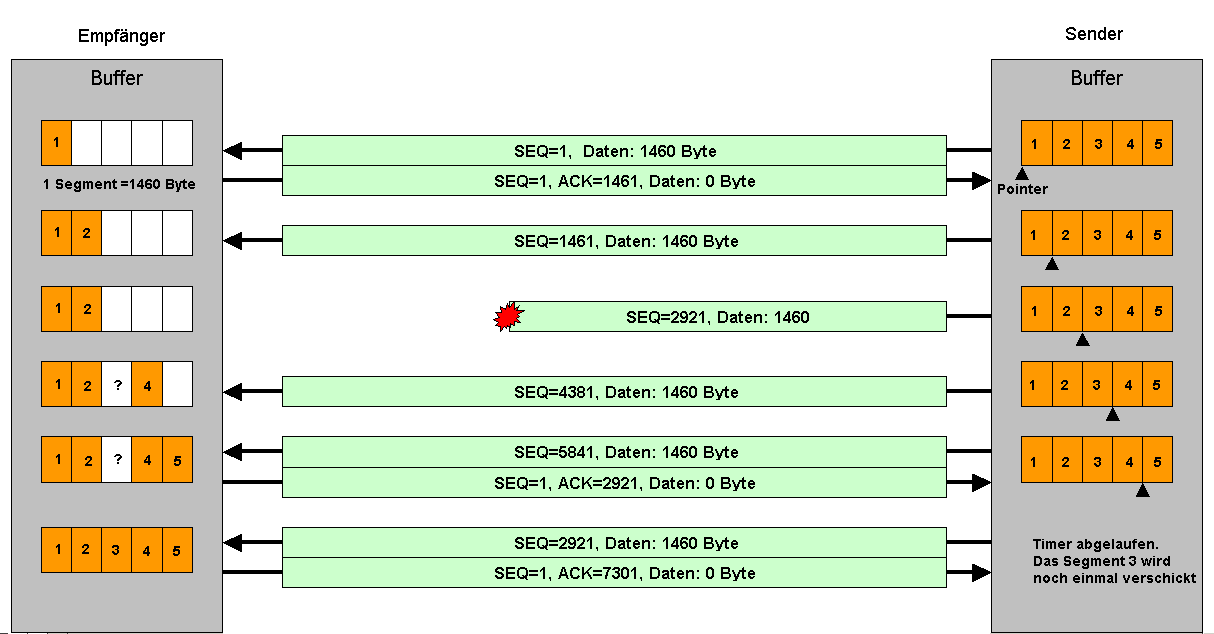
\includegraphics[width=\textwidth]{gfx/Tcp_transfer.png}
      \caption{TCP data Transmission with sequence numbers}
      \label{fig:tcp_data_transmission}
\end{figure}